%        File: covo.tex
%     Created: Di Okt 16 10:00  2018 C
% Last Change: Di Okt 16 10:00  2018 C
%

\documentclass[a4paper]{report}
% ***************************PACKAGES***************************
\usepackage{graphicx}
\usepackage{caption,setspace}
\usepackage{subcaption}
\captionsetup[figure]{width=0.7\textwidth,font={small}}
\usepackage{float}
\usepackage{amsmath}
\usepackage{amssymb}
\usepackage{hyperref}
\usepackage{siunitx}
\usepackage{graphicx}
\usepackage{subcaption}
\usepackage{mwe}
\usepackage{tabularx}
\usepackage{cite}
\usepackage{hyperref}
\usepackage{bookmark}
\usepackage{algorithm}
\usepackage[noend]{algpseudocode}


% ***************************CONFIGS***************************
% for numbering per section
\numberwithin{figure}{section}
% removing ugly colored rectangles from references
\usepackage{xcolor}
\hypersetup{
    hidelinks,
    colorlinks = false,
    %linkcolor={black},
    %citecolor={black},
    %urlcolor={black}
  }
% command for table tabular alignment
\newcolumntype{L}{>{\raggedright\arraybackslash}X}
% command for argmin and argmax
\DeclareMathOperator*{\argmax}{arg\,max}
\DeclareMathOperator*{\argmin}{arg\,min}
\newcommand{\R}{\mathbb{R}}
% commands for cascading subfigures
\newsavebox{\subfloatbox}
\newcommand{\topfloat}[2][\empty]% #1 = caption, #2=image
 {\savebox\subfloatbox{#2}%
  \begin{minipage}[t]{\wd\subfloatbox}
    \usebox\subfloatbox
    \subcaption{#1}
  \end{minipage}}
\newcommand{\bottomfloat}[2][\empty]% #1 = caption, #2=image
 {\savebox\subfloatbox{#2}%
  \begin{minipage}[b]{\wd\subfloatbox}
    \captionsetup{position=top}%
    \subcaption{#1}
    \usebox\subfloatbox
  \end{minipage}}

\algnewcommand\algorithmicforeach{\textbf{for each}}
\algdef{S}[FOR]{ForEach}[1]{\algorithmicforeach\ #1\ \algorithmicdo}

% ***************************ACRONYMS***************************
\usepackage[toc, shortcuts]{glossaries}
\makeglossaries
\newacronym{vo}{VO}{Visual Odometry}



\begin{document}

% ***************************TITLE***************************
\begin{titlepage}
\begin{center}

%  
\includegraphics[width=\textwidth]{../fig/tuc_logo.jpg}

\vspace{1.5cm}


{\Huge \textbf{Master Thesis}}\\
\vspace{0.5cm}
{\huge \textbf{An Error Aware RGB-D \\Visual Odometry}}


\vspace{2.5cm}

{\huge \textbf{U\u{g}ur Bolat}}

\vfill

Date:

\vspace{1.2cm}

Supervisors: \\
Dr.-Ing. Sven Lange \\
M.Sc. Tim Pfeifer

\vspace{0.8cm}

Faculty of Electrical Engineering and Information Technology\\
Professorship of Process Automation

\end{center}
\end{titlepage}

% ***************************TABLE OF CONTENT ETC.***************************
\tableofcontents
\newpage
\listoffigures
\listoftables
\newpage
\printglossary[type=\acronymtype,title={Abbreviations}]
\newpage

% ***************************DOCUMENT***************************

\begin{abstract}


\end{abstract}

\newpage

% ***************************CP1-INTRO***************************
\chapter{Introduction} \label{cp_intro}


\newpage

% ***************************CP2-VO***************************

\chapter{Camera Models} \label{cp_cam_models}

A camera maps from a 3D world scene to a 2D image plane. We call this process 
projection operation. Since the \acrshort{vo} systems process camera image 
sequences, one has to model this projection operation accurately. One of the 
basic camera modeling technique is the \textit{Pinhole Model} where the projection of 
the 3D points are mapped on a 2D image plane (also called focal plane). 

\subsection{The Pinhole Model} \label{sbsc_pinhole}

In this model, the camera centre sits behind the image plane.
The Z-axis, 
also called \textit{principal axis}, of this 
coordinate system points out through the origin of the image plane and the 
point where pierce through image plane is called the \textit{pricipal point}. 
We can also see how other two axes are located in Figure-\ref{fig:pinhole} 
and this is known as the \textit{Camera Coordinate System} $(x_{cam}, y_{cam}, z_{cam})$.


\begin{figure}[H]
	\centering
	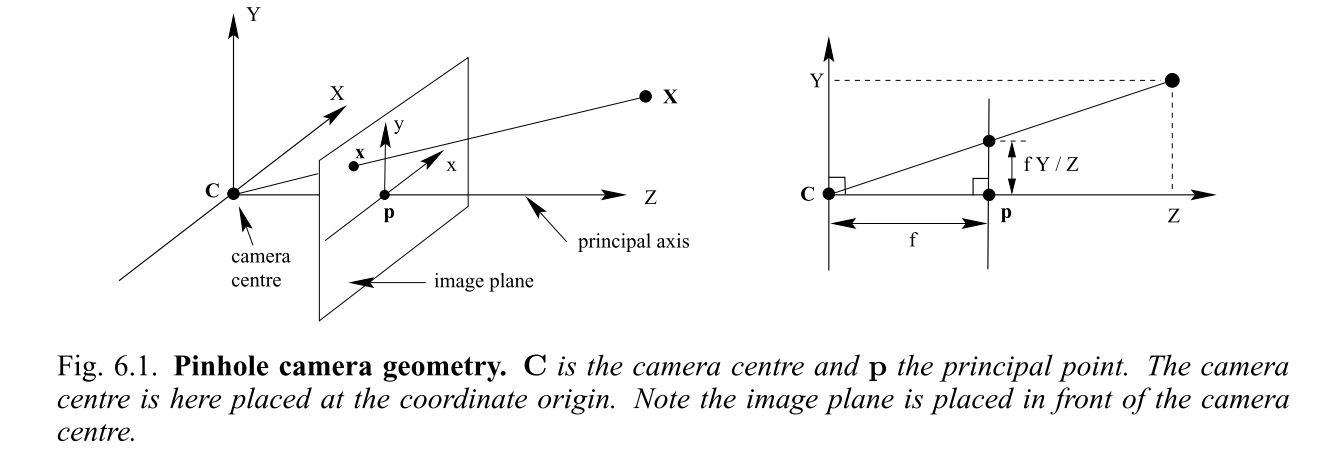
\includegraphics[width=\linewidth,natwidth=640,natheight=640]
  {fig/ref_imgs/pinhole_model.png}
  \caption{REMEMBER TO DRAW HORIZ/VERT Fx and Fy. The Pinhole Model}
	\label{fig:pinhole}
\end{figure}

Thanks to geometrical propotion property, we can project 
the 3D point $(X, Y, Z)^T$ in Euclidean space $\mathbb{R}^3$
to the 2D point $(U,V)^T = (f_xX/Z, f_yY/Z)^T$ in Euclidean space $\mathbb{R}^2$, 
where $f_x$ and $f_y$ are the \textit{focal lengths} 
between the camera centre and the pricipal 
point with respect to horizontal and vertical axis of the Camera Coordinate 
System respectively.
After projection, we obtain a 2D 
point that we represent on the 
\textit{Image Coordinate Frame} $(u_{img},v_{img})$.

To be more specific,
we can write the projection operation as a linear mapping function 
in the following way if we utilize the homogenous coordinates:

\begin{equation}
  \begin{pmatrix}
    U\\
    V\\
    1
  \end{pmatrix}
  \sim
  Z
  \begin{pmatrix}
    f_xX/Z\\
    f_yY/Z\\
    1
  \end{pmatrix}
  =
  \begin{pmatrix}
    f_xX\\
    f_yY\\
    Z
  \end{pmatrix}
  =
  \begin{bmatrix}
    f_x & 0 & 0 & 0\\
    0 & f_y & 0 & 0\\
    0 & 0 & 1 & 0\\
  \end{bmatrix}
  \begin{pmatrix}
    X\\
    Y\\
    Z\\
    1
  \end{pmatrix}
\end{equation} \label{eq:proj_func_w_f}

This equation applies for the case when 3D points are 
projected onto a plane where the principal point is the origin. 
However, the common convention in partice 
is to have the origin at the (not entirely sure) left-bottom corner not in the centre.

\begin{figure}[H]
	\centering
	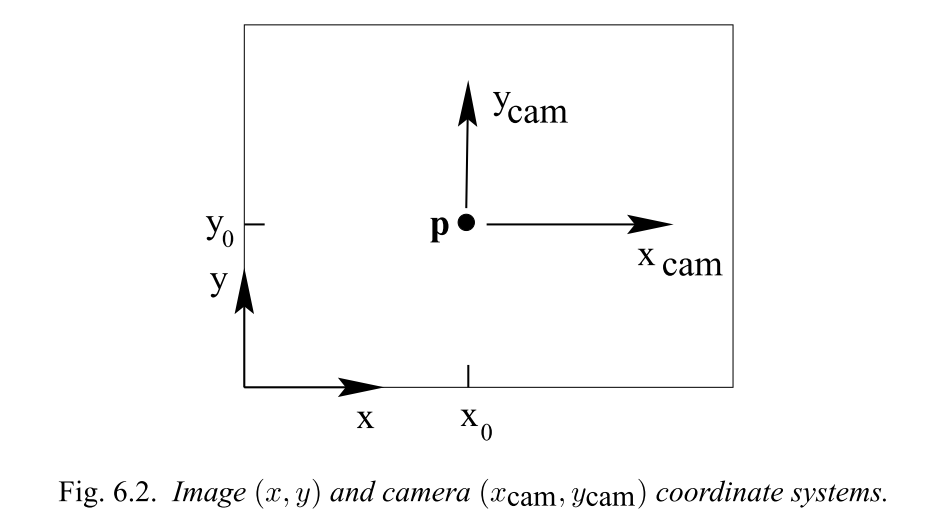
\includegraphics[width=\linewidth,natwidth=640,natheight=640]
  {fig/ref_imgs/pinhole_offset.png}
	\caption{Principle Point Offset}
	\label{fig:pinhole_offset}
\end{figure}

Thus, we get offsets, which can further be added into our function:

\begin{equation}
  \begin{pmatrix}
    U\\
    V\\
    1
  \end{pmatrix}
  \sim
  Z
  \begin{pmatrix}
    (f_xX + Z c_x)/Z\\
    (f_yY + Z c_y)/Z\\
    1
  \end{pmatrix}
  =
  \begin{pmatrix}
    f_xX + Z c_x\\
    f_yY + Z c_y\\
    Z
  \end{pmatrix}
  =
  \begin{bmatrix}
    f_x & 0 & c_x & 0\\
    0 & f_y & c_y & 0\\
    0 & 0 & 1 & 0\\
  \end{bmatrix}
  \begin{pmatrix}
    X\\
    Y\\
    Z\\
    1
  \end{pmatrix}
\end{equation} \label{eq:proj_func_w_f_c}

where $c_x$ and $c_y$ are coordinates of the principal point \textbf{p}.

In addition to pricipal offsets, inaccurately synchronized pixel-sampling 
process can result in \textit{skewed pixels}. This camera imperfection leads to 
non-square pixels as seen in Figure-\ref{fig:skewed}.

\begin{figure}[H]
	\centering
  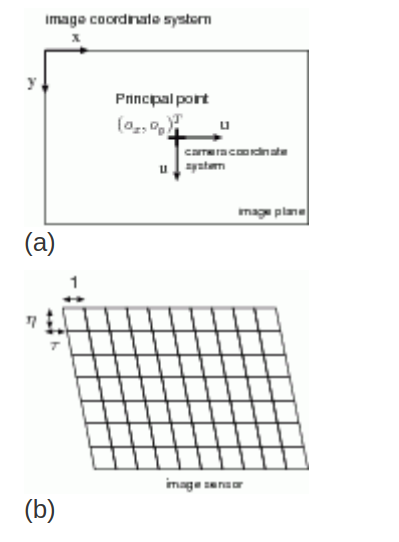
\includegraphics[width=0.5\linewidth,natwidth=640,natheight=640]
  {fig/ref_imgs/skew.png}
  \caption{REMEMBER TO DRAW FOR X and Y.Skew and Non-Square Pixels}
	\label{fig:skewed}
\end{figure}

We can scale the square pixels, having 1:1 pixel aspect ratio, with the 
corresponding skew parameters $\eta_x$, $\eta_y$ and $s$:

\begin{equation}
  \begin{pmatrix}
    U\\
    V\\
    1
  \end{pmatrix}
  \sim
  \begin{bmatrix}
    f_x\eta_x & s & c_x & 0\\
    0 & f_y\eta_y & c_y & 0\\
    0 & 0 & 1 & 0\\
  \end{bmatrix}
  \begin{pmatrix}
    X\\
    Y\\
    Z\\
    1
  \end{pmatrix}
  =
  \begin{bmatrix}
    \alpha_x & s & c_x & 0\\
    0 & \alpha_y & c_y & 0\\
    0 & 0 & 1 & 0\\
  \end{bmatrix}
  \begin{pmatrix}
    X\\
    Y\\
    Z\\
    1
  \end{pmatrix}
\end{equation} \label{eq:proj_func_w_square_pix_skew}

Generally, the skewed pixels issues occurred in ealier versions of CCD cameras 
and this is mostly fixed in new generation digital cameras. Therefore, 
we can neglate this effect by taking $\eta_x=1$, $\eta_y=1$ and $s=0$.

Next, we can extract:

\begin{equation}
  \mathbf{K} = 
  \begin{bmatrix}
    \alpha_x & s & c_x\\
    0 & \alpha_y & c_y\\
    0 & 0 & 1\\
  \end{bmatrix}
\end{equation} \label{eq:k_matrix}

The $\mathbf{K}$ matrix is called 
\textit{intrinsic parameters matrix}, which represents the characteristics of 
a camera sensor. Note that, we 
can further reformulate the notation \ref{eq:proj_func_w_square_pix_skew} in more 
compact form:

\begin{equation}
  \mathbf{x_{img}} = \mathbf{K}[\mathbf{I}|\mathbf{0}]\mathbf{X_{cam}}
\end{equation} \label{eq:simplyfied_proj_func}

\begin{figure}[H]
	\centering
  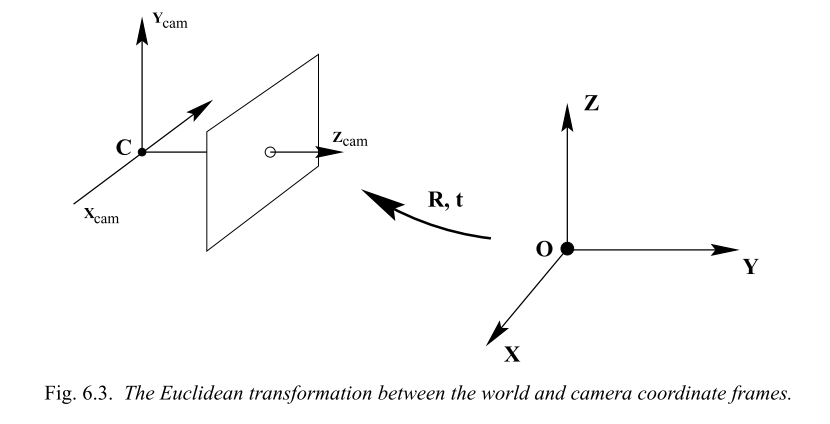
\includegraphics[width=\linewidth,natwidth=640,natheight=640]
  {fig/ref_imgs/cam_model_rot_trans.png}
  \caption{Camera Rotation and Translation}
  \label{fig:cam_model_rot_trans}
\end{figure}

Remember that, the Z-axis of the Camera Coordinate System aligns with the 
principal axis that is \textit{local} to camera frame. In fact, we have 3D points that 
we represent in the \textit{World Coordinate System} 
which we refer as the \textit{global} frame. 
These two coordinates systems 
can be transformed one another by a rotation and a translation as it is 
depicted in Figure-\ref{fig:cam_model_rot_trans} but we are interested in 
converting from the World Coordinate to Camera Coordinate System in this case.
To do so, we first perform series of rotations around each axis of the 
cartesian coordinate system in Euclidean space by using 
\textit{rotation matrices} where $R_x, R_y, R_z \in SO(3)$ is the rotation group:

\begin{equation}
  R_x(\theta) = 
  \begin{bmatrix}
    1 & 0 & 0\\
    0 & cos\theta & -sin\theta\\
    0 & sin\theta & cos\theta
  \end{bmatrix}
\end{equation} \label{eq:rot_matrx_x}

\begin{equation}
  R_y(\theta) = 
  \begin{bmatrix}
    cos\theta & 0 & -sin\theta\\
    0 & 1 & 0\\
    sin\theta & 0 & cos\theta
  \end{bmatrix}
\end{equation} \label{eq:rot_matrx_y}

\begin{equation}
  R_z(\theta) = 
  \begin{bmatrix}
    cos\theta & -sin\theta & 0\\
    sin\theta & cos\theta & 0\\
    0 & 0 & 1
  \end{bmatrix}
\end{equation} \label{eq:rot_matrx_z}

One can concatenate all three rotations about axes z, y, x respectively:

\begin{equation}
  \mathbf{R} = \mathbf{R_z(\gamma)}\mathbf{R_y(\beta)}\mathbf{R_x(\alpha)}
  =
  \begin{bmatrix}
    r_{11} & r_{12} & r_{13}\\
    r_{21} & r_{22} & r_{23}\\
    r_{31} & r_{32} & r_{33}\\
  \end{bmatrix}
\end{equation} \label{eq:rot_matrix_derivation}

Then, perform a translation $\mathbf{t} \in \R^{3x1}$:

\begin{equation}
  \mathbf{t} = 
  \begin{bmatrix}
    t_x \\ t_y \\ t_z
  \end{bmatrix}
\end{equation} \label{eq:translation}

We can also compound the rotation matrix and the translation vector into 
one matrix:

\begin{equation}
  \mathbf{T} =
  \begin{bmatrix}
    r_{11} & r_{12} & r_{13} & t_x\\
    r_{21} & r_{22} & r_{23} & t_y\\
    r_{31} & r_{32} & r_{33} & t_z\\
  \end{bmatrix}
\end{equation} \label{eq:transformation_matrix}

The $\mathbf{T} \in \R^{4x3}$ matrix in fact represents 
a \textit{rigid-body transformation}, which we call 
\textit{extrinsic camera parameters}.

Finally, we combine intrinsic $\mathbf{K}$ and 
extrinsic $\mathbf{T}$ matrices to form the following notation: 

\begin{equation}
  \mathbf{x_{img}} = 
  \mathbf{P}\mathbf{X_{world}} = 
  \mathbf{K}\mathbf{T}\mathbf{X_{world}} = 
  \mathbf{K}[\mathbf{R}|\mathbf{t}]\mathbf{X_{world}}
\end{equation} \label{eq:simplyfied_proj_func}

\begin{equation}
  \mathbf{x_{img}} = \mathbf{F_{proj}}(\mathbf{X_{world}})
\end{equation} \label{eq:simplyfied_proj_func}

where $\mathbf{F_{proj}}(\mathbf{X_{world}})$ is the 
\textit{projective transformation function}, which takes 
the 3D points in the World Coordinate System, transforms to 
the Camera Coordinate Systems and then maps them into the Image 
Coordinate Systems.

To build any reliable computer vision application with digital cameras, it is 
to important to find a good $\mathbf{P}$ \textit{projection matrix}. 
The next section describes one of many numerical methods for estimationg this 
matrix in literature.

\section{Camera Calibration} \label{sb_sc_calibration}


It is important to note that derivations of the formulation of this section
is not provided. Therefore, I refer readers to \cite{bla} for the detailed 
formulation. However, the intiution of the calibration process is fairly 
straightforward. 

\begin{figure}[H]
	\centering
  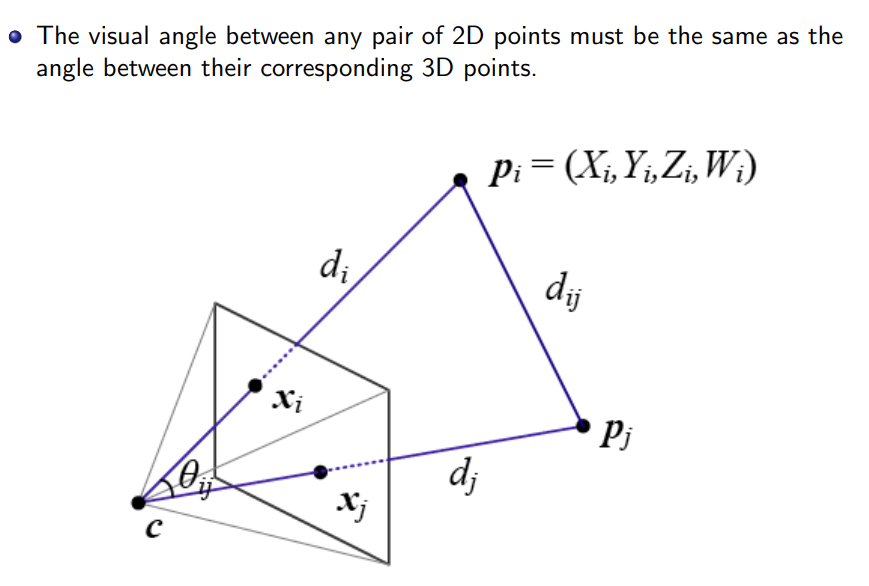
\includegraphics[width=\linewidth,natwidth=640,natheight=640]
  {fig/ref_imgs/calibration_dlt.png}
  \caption{Inheret Constraint}
  \label{fig:calibration_constraint}
\end{figure}


Assuming that we project two 3D points onto our image plane
like in Figure-\ref{fig:calibration_constraint},
the visual angle between those pair of 3D points is equal to 
the angle between its corresponding 2D points. This geometric constraints 
allow us to build the calibration problem. Remember that the goal is to find 
the projection matrix and we can build the problem in the following way:

\begin{equation}
  \mathbf{x_{img}} = 
  \begin{pmatrix}
    u_i\\
    v_i
  \end{pmatrix}
  =
  \mathbf{P}\mathbf{X_{world}} = 
  \begin{bmatrix}
    p_{00} & p_{01} & p_{02} & p_{03}\\
    p_{10} & p_{11} & p_{12} & p_{13}\\
    p_{20} & p_{21} & p_{22} & p_{23}
  \end{bmatrix}
  \begin{pmatrix}
    X_i\\
    Y_i\\
    Z_i\\
  \end{pmatrix}
\end{equation} \label{eq:simplyfied_proj_func}

After elaborating notation \ref{eq:simplyfied_proj_func}, let's distribute 
the projection matrix onto the 3D point measurement to retrieve individual 
pixel coordinates:

\begin{equation}
  u_i = 
  \frac
  {p_{00}X_i + p_{01}Y_i + p_{02}Z_i + p_{03}}
  {p_{20}X_i + p_{21}Y_i + p_{22}Z_i + p_{23}}
\end{equation} \label{eq:u_i}

\begin{equation}
  v_i = 
  \frac
  {p_{10}X_i + p_{11}Y_i + p_{12}Z_i + p_{13}}
  {p_{20}X_i + p_{21}Y_i + p_{22}Z_i + p_{23}}
\end{equation} \label{eq:v_i}


Since $\mathbf{x_{img}}$ and $\mathbf{X_{world}}$ are known,
we can find elements of the $\mathbf{p} = (p_{00}, p_{01}, \dots, p_{23})^T$ matrix 
by solving $\mathbf{Ap=0}$ liner system of equations from \ref{eq:u_i} and \ref{eq:v_i}.

For \textit{minimal solution} of this linear system of equations, 
we need at least $n \geq 6$ measurement points to solve the problem as 
the $\mathbf{P}$ matrix has 12 degree of freedom (11 if scale is ignored).
Note that this accounts for having 
noise-free measurement which does not hold in reality. Then, the problem 
becomes \textit{over-determined}.

In noisy measurement case, the problem is usually solved with
\textit{singular value decomposition (SVD)} with $n \geq 6$ measurement points. 
This method is called the \textit{Direct Linear Transformation (DLT)}.
Disadvantange of the DLT methods, it is still sensitive errors since 
it only considers \textit{algebraic errors}, which are the residuals of 
$\mathbf{Ap}$. 

While estimating the intrinsic and extrinsic parameters 
that are in linear form with the DLT, 
another issue known as \textit{radial distortion} 
has to take into account as well. This issue is caused by camera lens 
and Figure-\ref{fig:cam_distortion} depicts this effect and the straight lines 
appear to be curved. 

\begin{figure}[H]
	\centering
  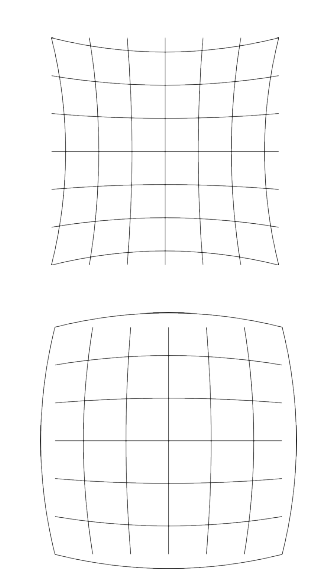
\includegraphics[width=0.3\linewidth,natwidth=640,natheight=640]
  {fig/ref_imgs/cam_distortion.png}
  \caption{Camera Distortion}
  \label{fig:cam_distortion}
\end{figure}

This distortion has non-linear characteristics and we also 
need to estimate the coefficients 
$\kappa = (k_1, k_2, p_1, p_2, k_3)^T$ of the following polynomial:


\begin{equation}
\begin{split}
  x''_i = F_{dist}(x') = 
  x'(1+ k_1 r^2 + k_2 r^4 + k_3 r^6) + 2 p_1 x' y' + p_2 (r^2+2x'^2)\\
  y''_i = F_{dist}(y') = 
  y'(1+ k_1 r^2 + k_2 r^4 + k_3 r^6) + p_1 (r^2+2y'^2) + 2p_2 x'y'\\
\end{split}
\end{equation}

where $x' = X_{cam}/Z_{cam}$ and $y' = Y_{cam}/Z_{cam}$. 
Note that, in \ref{eq:simplyfied_proj_func}, we first transform 
3D points from World Coordinate to Camera Coordinate Systems with 
extrinsic matrix and then we project them with the instrinsic matrix. 
To improve our pinhole camera model, 
we need to distort 3D points in the Camere Coordinate System before 
multiplying with the intrinsic matrix:

\begin{equation}
  \begin{pmatrix}
    U\\
    V\\
    1
  \end{pmatrix}
  =
  \begin{pmatrix}
    f_x x'' + c_x\\
    f_y x'' + c_y\\
    1
  \end{pmatrix}
    =
    F_{dis}\begin{pmatrix}
      \mathbf{K}
      \begin{pmatrix}
        X_{cam}\\
        Y_{cam}\\
        Z_{cam}\\
        1
      \end{pmatrix}
    \end{pmatrix} 
    =
    F_{dist}\begin{pmatrix}
      \mathbf{K} [\mathbf{R}|\mathbf{t}]
      \begin{pmatrix}
        X_{world}\\
        Y_{world}\\
        Z_{world}\\
        1
      \end{pmatrix}
    \end{pmatrix}
\end{equation} \label{eq:proj_func_w_f_c}

Above operations introduce non-linearity, which cannot be solved by DLT.
To get better accuracy at our projection matrix along with the distortion, 
\textit{least squares estimation}, i.e., Levenberg-Marquardt, is perfomed.

\begin{figure}[H]
	\centering
  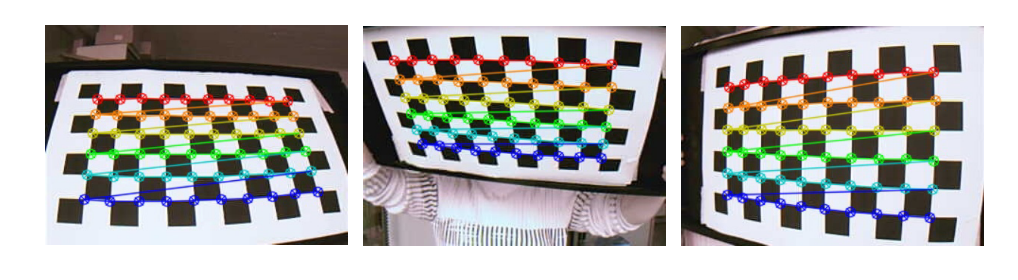
\includegraphics[width=\linewidth,natwidth=640,natheight=640]
  {fig/ref_imgs/checkerboard.png}
  \caption{Checkerboard}
  \label{fig:checkerboard}
\end{figure}

In practice, the checkerboard is used to get many good measurement points 
as  we easily extract edge features from the image. Now, the DLT comes handy
as we can use the DLT's result as an initial guess 
in the least squares optimization problem.

\begin{equation}
  \argmin_{\mathbf{p} \rightarrow \mathbf{K}, \kappa, \mathbf{R}_i, \mathbf{t}_i}
  \sum_{i=1:n} || \mathbf{x_{i}} - 
  \mathbf{P} \mathbf{X_{i}} ||^2
\end{equation}

where $\mathbf{K}$ is the intrinsic matrix, 
$\kappa$ is the distortion coefficients, 
$\mathbf{R_i}$ is the corresponding orientation and 
$\mathbf{t_i}$ is the corresponding translation.
The afromentioned calibration process is well-studied problem in literature. 
Fortunately, there are many software libraries, such as OpenCV, 
that offers such implementations.



\chapter{Visual Odometry} \label{cp_vo}

\section{Image Features} \label{sc_img_features}

Image features are a collection of regions of interest or of points of interest 
that describe the image. In this way, we compress the necessary information 
from images so that we can achieve computationaly expensive task more efficiently.
Points of interest, also called \textit{keypoints}, 
are particularly valuable because their location in the image can be 
measured accurately. This is useful for localization related tasks such as VO. 

\subsection{Feature Extraction} \label{sb_sc_feature_extraction}

Generally, the goal is to find good features in feature-based VO. 
What defines a good feature is that it must be distinct, 
repeatable, computationaly cheap and invariant to geometrical changes. 
Obviously, one has many options to produce such image 
feautes but two common methods that are widely used in VO systems are 
blobs and corners. 
Blobs are image patterns that contain distinct image response comparing to their 
neighborhood pixels. Blobs take advantage of pixel intensity or color to 
decide whether it has a distinct response or not.
In the VO literature, SIFT\cite{}, SURF\cite{} or CENSURE\cite{} are popular 
choices for detecting blob featurus.
Corners are the meeting points where two or many edges intersect. Corners 
take advantage of geometrical structure of an image. FAST\cite{}, Shi-Tomasi or 
Haris\cite{} are widely used for detecting corners.

Fundemantally, a two-step process is needed to extract good features. 
First, you take a response function, called \textit{image filter}, 
shift this filter through the image and save the one that have greater 
response than your previously defined threshold as Keypoints.
In blob case, this might a Gaussian filter or a 
corner detector filter in corner case. Second, you perform non-maxima 
suppression on the resulting keypoints to find local minima of the function. 
The second step ensures you get keypoints only with maximum confidence. 

Inheritly, each feature detector has certain limitations and one has to 
choose whihc detector to use according to task objectives. Therefore, one can ask 
does the localization envorinment involve more texture oriented objects like 
floors, walls etc. or geometrical shapes like urban areas where many lines 
exist?
However, rule of thumb when choosing feature detector is that blobs 
are distinct but slow to compute and corners are fast to compute but less 
distict. 

\subsection{Feature Descriptor} \label{sb_sc_feature_descriptor}

Extracting features is the very first step of VO. The next step is to 
encode the detected keypoints into a format that we can perform comparison 
or search operation among them. This is done by taking the neighboring pixels 
around the keypoints and convert into a more compact form. For example, SIFT 
creates a patch around a keypoint, divides this patch into smaller grids,
calculate the gradient of each grid and 
saves into a histogram form.
This procedure makes feature descriptor 
robust agaist scale or rotation changes. Then, one can use these descriptors for 
various comparison operations such as matching or tracking in VO.


\subsection{ORB} \label{sb_sc_orb}

One of the most strict requirements of VO is the real-time contraints since it is 
expected to work at similari to low-sensors, i.e., accelerometer, gyroscopes etc. 
As previously discussed, blobs detectors are computationaly expensive. Therefore, 
corners based feature detector are more prevelant in VO. 
\textit{ORB (oriented FAST and rotated BRIEF)} studied known issues of 
FAST detector and BRIEF descriptor. Then, it fixed them into a level that 
it perform as accurate as SIFT, plus faster. Here are steps on how to extract features 
and create descriptors with ORB: 

\begin{enumerate}
  \item \textbf{Detect corners with FAST}: FAST take each pixel on 
    the image and compare with its adjacent pixels. More specificially, 
    ORB uses FAST-9, which takes a patch of discrete circular radius of $r=9$. 

    \begin{figure}[H]
	\centering
  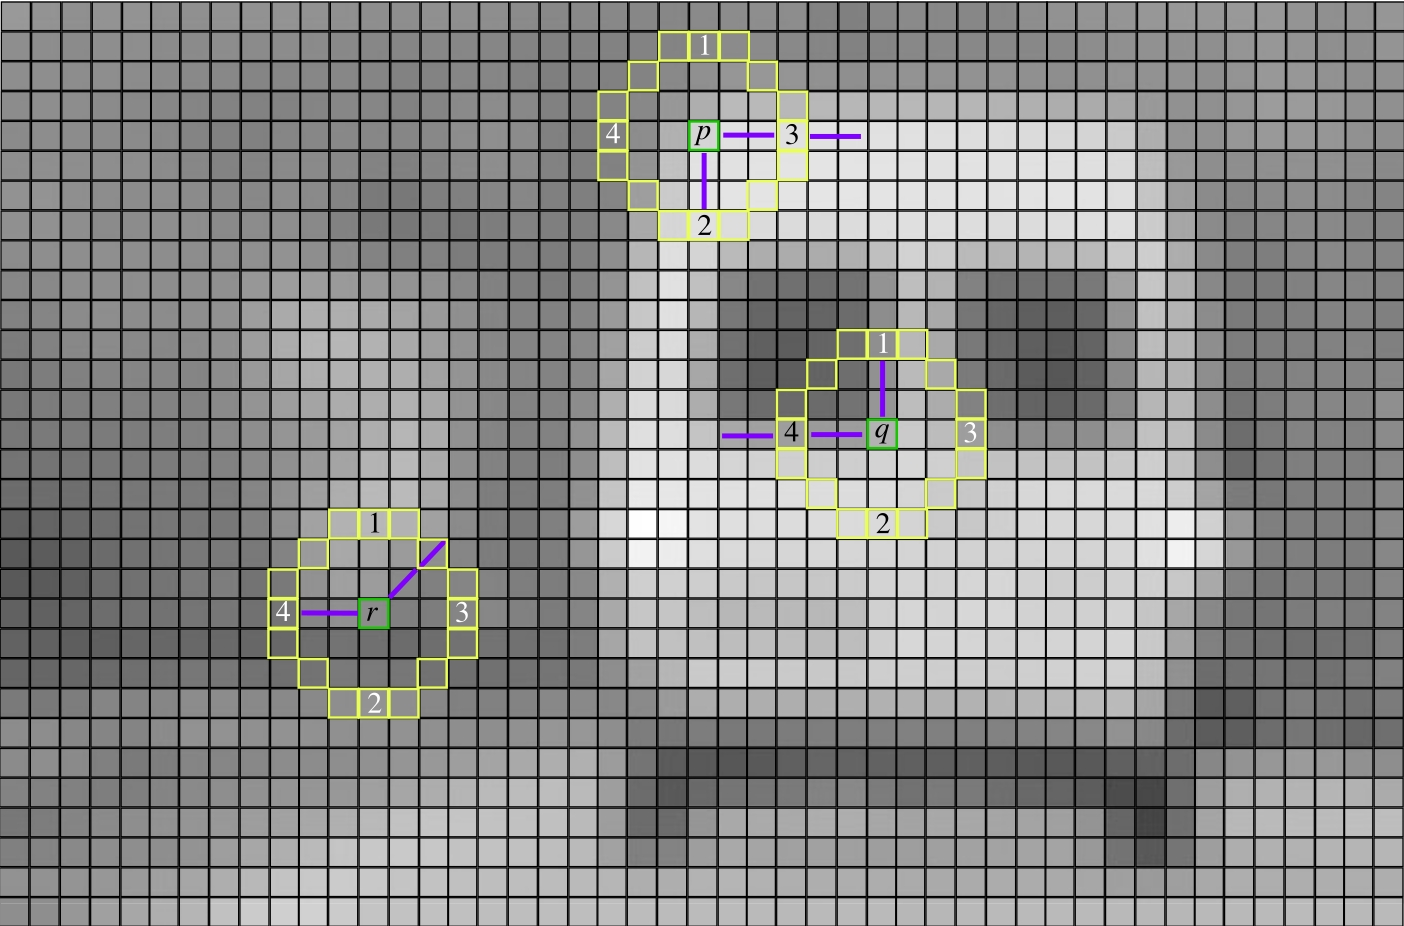
\includegraphics[width=0.6\linewidth,natwidth=640,natheight=640]
  {fig/ref_imgs/fast.png}
  \caption{FAST corners}
  \label{fig:fast_corners}
\end{figure}

    If the 
    selected pixel is $\pm t$ darker or brighter than adjacent pixels, 
    we call it a corner, where $t$ is our empiric threshold.

\begin{equation}
  M_c(p) = 
  \sum_{r \in S_{bright}} |I_{p \rightarrow r} - I_p| - t \text{ or } 
  M_c(p) = 
  \sum_{r \in S_{dark}} |I_p - I_{p \rightarrow r}| - t)
\end{equation}
    We retrieve $M^c_{1:n}$ the set of corner candidates from 
    comparing $I_{p\rightarrow x}$ the adjacent pixels around $I_p$ the target pixel.

  \item \textbf{Rank detected keypoint with Harris}: After FAST detection, 
    we get many corner candidates around the interest point. However, 
    FAST does not measure how good a corner is. Thus, we use Harris corner 
    detector to rank corner candidates:
    \begin{equation}
      \mathbf{A} = \sum_{x,y} w(x,y) 
      \begin{bmatrix}
        I_x^2 & I_xI_y \\ I_xI_y & I_y^2
      \end{bmatrix}
    \end{equation}
    The $\mathbf{A}$ matrix is calculated by the $I_x$ and $I_y$ partial 
    derivatives with respect to x and y direction and $w(x,y)$ weighting window.

    \begin{equation}
      R^c = det(\mathbf{A}) - k(trace(\mathbf{A}))^2
    \end{equation}
    where $det(\mathbf{A}) = \lambda_1 \lambda_2$ and 
    $trace(\mathbf{A}) = \lambda_1 + \lambda_2$.
    Then, we use the resulting $\mathbf{A}$ to find a ranking score for each 
    corner. Now, it is possible to take top N corners if desired.

  \item \textbf{Calculate orientation of corners with image moments}: 
    ORB uses BRIEF to create feature descriptors; however, BRIEF fails in 
    rotated images. Therefore, ORB modifies the BRIEF by adding orientation 
    information. To get orientation, an \textit{image moment} are calculated
    for each patch $S$:

    \begin{equation}
      m_{a,b}(S) = \sum_{x,y \in S} x^a y^b I(x,y)
    \end{equation}
    where $a + b$ defines the order of the moment and we need 
    the moments of order one:

    \begin{equation}
      m_{1,0}(S) = \sum_{x,y \in S} x \cdot I(x,y) \text{  ,  }
      m_{0,1}(S) = \sum_{x,y \in S} y \cdot I(x,y)
    \end{equation}

    Then, we get the orientation of the patch S:
    \begin{equation}
      \theta(S) = atan2(m_{01}, m_{10})
    \end{equation}

  \item \textbf{Form BRIEF descriptors with their corresponding orientation}:
    Once the top N corners and their orientations are detected, descriptions 
    can be formed with BRIEF. 

\begin{figure}[H]
	\centering
  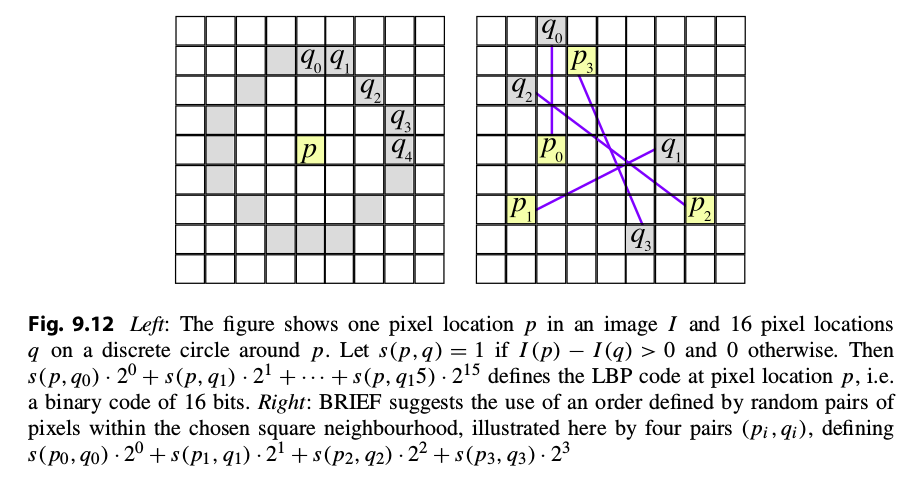
\includegraphics[width=\linewidth,natwidth=640,natheight=640]
  {fig/ref_imgs/brief.png}
  \caption{BRIEF pairs}
  \label{fig:brief_pairs}
\end{figure}


    To do so, we randomly (generated by normal distribution) 
    selected 256 pairs $(p_i,q_i)$ 
    inside the patch $S$:
    \begin{equation}
      \mathbf{S} = 
      \begin{pmatrix}
      p_0, \dots, p_n\\
      q_0, \dots, q_n
      \end{pmatrix}
    \end{equation}
    Next, we rotate each $(\mathbf{p_i, q_i})$ pair points in 
    $\mathbf{S}$ with the 
    corresponding corner's orientation:
    \begin{equation}
      \mathbf{p}_{i,\theta} = \mathbf{R}_{\theta}\mathbf{p_i} \text{ and } 
      \mathbf{q}_{i,\theta} = \mathbf{R}_{\theta}\mathbf{q_i}
    \end{equation}
    where $p_i=(x_i, y_i)$ and $q_i=(x_i, y_i)$ are the pixel coordinates of 
    the points.
    It is important to note that authors \cite{} suggested to rotate each point in 
    increments of 2$\pi$/30. Therefore, orientaion $\theta$ is mapped to 
    nearest multiple of 2$\pi$/30.

    To form steered (or rotated) BRIEF descriptors, we perform pixel density comparison:
    between randomly selected pair points:
    \begin{equation*}
      \tau(\mathbf{p_{i,\theta}},\mathbf{q_{i,\theta}}) := 
      \begin{cases}
        1  & I(\mathbf{p_{i,\theta}}) < I(\mathbf{q_{i,\theta}}),\\
        0  & I(\mathbf{p_{i,\theta}}) \geq I(\mathbf{q_{i,\theta}})
      \end{cases}
    \end{equation*}

    Finally, we sum comparison results with binary form to get the desctriptor 
    of the patch $S$:
    \begin{equation}
      f(S) := \sum_{1\leq i \leq n} 2^{i-1}\tau (\mathbf{p_{i,\theta}, q_{i,\theta}})
    \end{equation}

\end{enumerate}





\section{Feature Matching} \label{sc_feature_matching}

\subsection{Brute-Force or FLANN} \label{sb_sc_}

\subsection{RANSAC} \label{sb_sc_ransac}

In reality, not all feature matches are correct and it is critical that we 
detect wrong ones as Least-Squares optimization that estimates the camera 
motion is sensitive to even small number of wrong matches. More technically,
we call these 
wrong matches \textit{outliers} (or \textit{false positives}). Hence, 
we need an algorithm to reject those outliers from \textit{inliers}. 
The most common way is to use RANSAC, which is an abbreviation to 
Random Sample Consensus. RANSAC is an interative algorithm which 
fits desired model with presence of outliers by selecting subset of dataset 
randomly and improving parameters of model each iteration. Note that 
RANSAC works 
well if at least half of the dataset contains inliers. 

\begin{figure}[H]
	\centering
	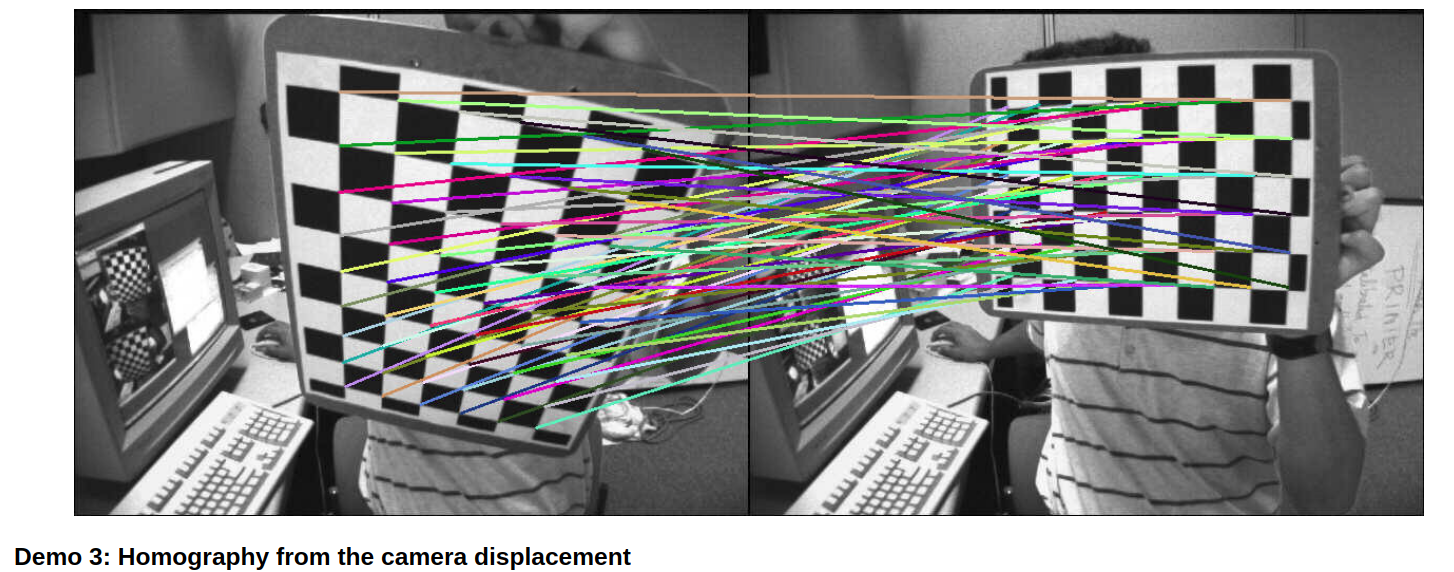
\includegraphics[width=\linewidth,natwidth=640,natheight=640]
  {fig/ref_imgs/outlier_matches.png}
  \caption{Outlier Mathces}
	\label{fig:outlier_matches}
\end{figure}

In \ref{sb_sc_calibration}, we discuss how to model rotation and translation 
behavior along with the intrinsic matrix. Parameteres that we aim to 
identify are elements of projection matrix in \ref{eq:proj_func_w_square_pix_skew}. 
Similarly, the model being fitted in RANSAC case is elements of a 
\textit{homography matrix}, 
which translates and rotates a point.
Remember that we have feature matches from image pairs. One of the pair is 
the translated and the rotated version of the other pair. 
We can 
model this relationship in the following way:

\begin{equation}
  k
  \begin{bmatrix}
    u' \\ v' \\1
  \end{bmatrix}
  =
  \mathbf{H}
  \begin{bmatrix}
    u \\ v \\1
  \end{bmatrix}
  =
  \begin{bmatrix}
    h_{00} & h_{01} & h_{02} \\
    h_{10} & h_{11} & h_{12} \\
    h_{20} & h_{21} & h_{22}
    \end{bmatrix}
  \begin{bmatrix}
      u \\ v \\1
    \end{bmatrix}
\end{equation}

select random subset

minize with lsq

check outside S and T


\begin{algorithm}[H]
  \caption{Rejecting outlier matches with RANSAC}\label{algo_ransac}

  \textbf{Input} \\
    \hspace*{\algorithmicindent}\textbf{S}: the smallest number of points\\
    \hspace*{\algorithmicindent}\textbf{N}: the number of iteration\\
    \hspace*{\algorithmicindent}\textbf{d}: the threshold used to identify a point which fits the model\\
    \hspace*{\algorithmicindent}\textbf{T}: the number of nearby points to notify that there is a good fit\\
  \textbf{Output} \\
    \hspace*{\algorithmicindent}\textbf{C}: the (consensus) set of inliers \\
  \begin{algorithmic}[1]

    \Procedure{RANSAC}{\textbf{S,N,d,T}}\\
      \While{iterations $<$ \textbf{N}}
      \State select random sample subset of \textbf{S} points
      \State estimate parameters to fit homography with \textbf{S}
      \ForEach {points outside \textbf{S}}
        \State calculate error between estimated point and measured point
        \If {error $<$ \textbf{d}}
          \State add point into \textbf{S}
        \EndIf
        \If {\textbf{S} $>$ \textbf{T}}
          \State return \textbf{C} $=$ \textbf{S}
        \EndIf
      \EndFor
      \EndWhile
    \EndProcedure
  \end{algorithmic}

\end{algorithm}

It is also important 
to note that estimated homography matrix corresponds the rotation and the 
translation that we need to calculate camera's trajectory. However, 
estimated homography matrix with the presence of outliers is not sufficient 
enough. Therefore, further optimization with is required to get more 
accurate rotation and translation with only inliers. We will discuss this 
optimization in the next section.


\section{Motion Estimation} \label{sc_motion_estim}

% ***************************CP3-MOTIVATION***************************
\chapter{Motivation} \label{cp_motivation}

% ***************************CP4-CoVO***************************
\chapter{An Error-Aware RGB-D Visual Odometry} \label{cp_covo}

REMEMBER TO DRAW X,Y COORD. WRT CAM. COORD WITH RIGHT HAND FOR KINECT!

\section{Modeling Spatial Uncertainty} \label{sc_spatial_uncertainty}

\subsection{Kinect Calibration} \label{sb_sc_kinect_calibration}

\section{Weighted Least-Squares Optimization} \label{sc_weighted_lsq}

\section{Covariance Estimation} \label{sc_covariance_estim}

% ***************************CP5-EVALUATION***************************
\chapter{Evaluation} \label{cp_evaluation}

% ***************************CP6-CONCLUSION***************************
\chapter{Conclusion} \label{cp_conc}

% ***************************CP7-EVALUATION***************************
\chapter{Reference} \label{cp_ref}


% ***************************CP7-EVALUATION***************************
\chapter{Appendices} \label{cp_appendices}

\section{Rigid-Body Transformations} \label{sc_rigid_body_transformations}

\end{document}


